\chapter{陈省身微分几何讲义}\index{陈省身微分几何讲义}
\section{流形的基本概念}\index{流形的基本概念}
\begin{thm}
\begin{enumerate}[label=(\arabic*),font=\upshape]
    \item 给定 $M,N$ 为两个 $n$维光滑流形且 $f$是从 $M$到 $N$的光滑映射.\cite{吴大任1979微分几何讲义}
    \item 在 $M$上一点 $p$处, $f$诱导的切映射 $f_*\colon T_p (M)\to T_{f(p)}(N)$是同构.
\end{enumerate}
则存在一点$p$在 $M$中的邻域 $U$, 使得 $V=f(U)$为 $f(p)$在 $N$中一邻域且 $f|_U\colon U\to V$是可微同胚.
\end{thm}
\begin{proof}
    由于 $f:M\to N$ 是光滑映射.故取 $p$在 $M$中局部坐标系 $(U_),\varphi)$和 点 $q=f(p)$在 $N$中局部坐标系 $(V_0,\psi)$,使得 $f(U_0)\subseteq V_0$,且
    \begin{eq*}
        \tilde{f}=\psi\circ f \circ \varphi^{-1}\colon \varphi (U_0)\to \psi (V_0) \subset \R^n.
    \end{eq*}
    是光滑映射.
    \begin{figure}[h]
        \begin{small}
            \begin{center}
                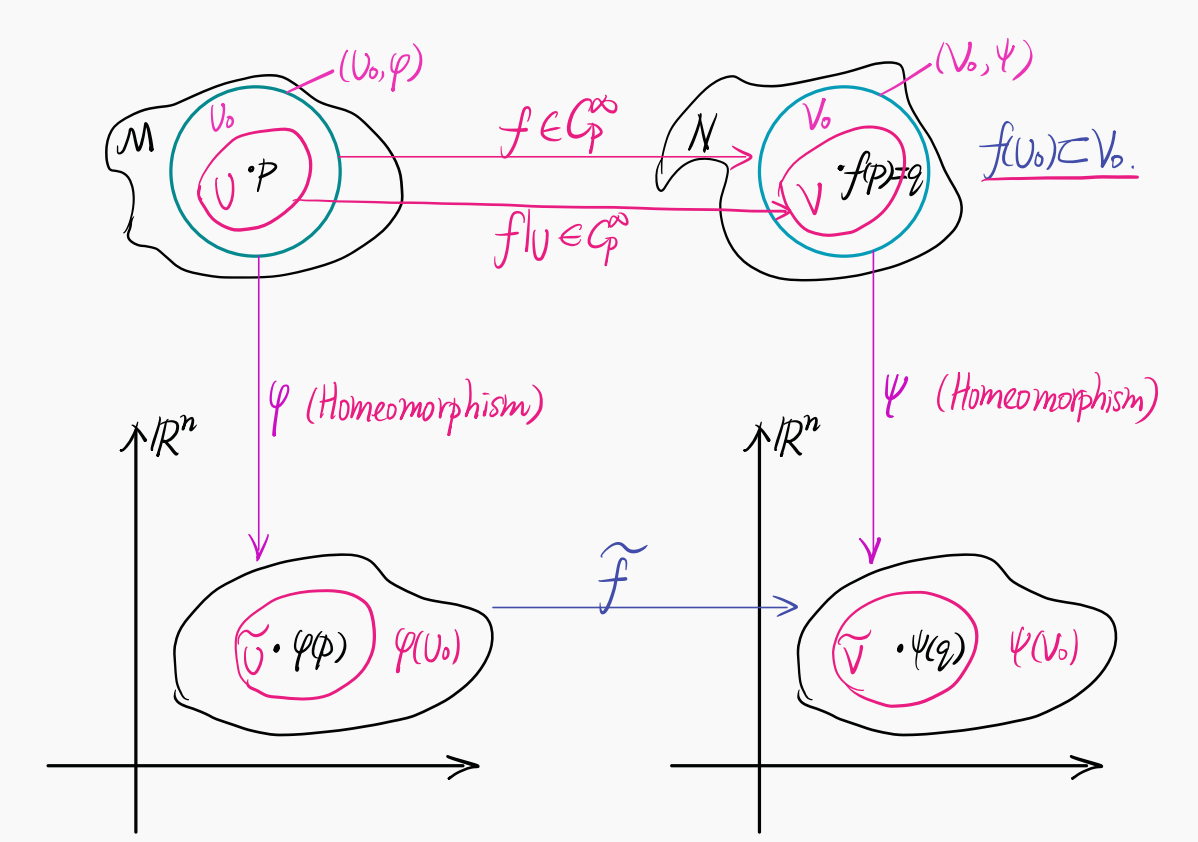
\includegraphics[width=0.6\textwidth]{figures/thm3.4.png}
            \end{center}
            \caption{图示}
            \label{fig:thm3.4proof}
        \end{small}
    \end{figure}
    
    故 $\tilde{f}=\psi\circ f\circ \varphi^{-1}$是光滑的. $\varphi(U_0)$与 $\psi(V_0)$均是 $\R^n$中的开集.在定理3.1中,令 $x_0=\varphi(p),f=\tilde{f}$,则若 $\det \left(\frac{\partial f^i}{\partial x^j}\right)\bigg|_{x_0}\neq 0$,则存在 $\varphi(p)$与$\psi(q)$在 $\varphi(U_0)$与 $\psi(V_0)$的邻域 $\widetilde{U}$与 $\widetilde{V}$,使得 $\tilde{f}|_{U_0}\colon \widetilde{U}\to\widetilde{V}$是可微同胚.

    令 $U=\varphi^{-1}(\widetilde{U}),V=\psi^{-1}(\widetilde{V})$,则 $U$与 $V$分别是$p$与 $q$在 $M$与 $N$中的邻域,且$f|_{U}=\psi^{-1}\circ \tilde{f}\circ \varphi\colon U\to V$是可微同胚.

    为何 $\tilde{f}$在 $\varphi(p)$的Jacobi行列式非零是显然的?
    由于
    \[
    \begin{aligned}
        & \left.\operatorname{det}\left(\frac{\partial f^i}{\partial x^j}\right)\right|_{x_0} \neq 0 . \Leftrightarrow f_*: T_{x_0} M\left(\simeq \mathbb{R}^n\right) \longrightarrow T_{f_{(x_0)}}\left(\mathbb{R}^n\right)\left(\simeq \mathbb{R}^n\right) \\
        & \left.\operatorname{det}\left(\frac{\partial \tilde{f}^i}{\partial x^j}\right)\right|_{\varphi(p)} \neq 0 \Leftarrow \tilde{f}_*: T_{\varphi(p)} M \left(\simeq \mathbb{R}^n\right) \longrightarrow T_{\tilde{f} \varphi(\rho)}\left(\mathbb{R}^n\right) (\simeq \mathbb{R}^n) 
        \end{aligned}\]
        故映射 $f$的 Jacobi矩阵 $\left(\frac{\partial f^i}{\partial x^j}\right)$恰是 $f_*$在自然基底下的矩阵.
\end{proof}
\subsection{小结}
\subsubsection*{余切空间}
\begin{itemize}
    \item 余切空间 $T^*_p =\F_p/\mathcal{H}_p=\{(\dd f)_p\}$,
    \item 自然基底 $\{(\dd u^i)_p,1\leqslant i\leqslant n\}$,
    \item 余切空间之间的光滑映射:
    \[F^*\colon T^*_q\to T^*_p\; \text{(设 $F\colon M\to N$是光滑映射且 $q=F(p)$.)}\]
    \begin{itemize}[label=\twicecircle]
        \item 作用方式 \quad $(\dd f)_p\mapsto \dd(f\circ F)$,
        \item 在两个自然基底下的矩阵表示: 
        
        设 $u^i$是 $p$附近的局部坐标表示, $v^\alpha$是 $q$附近的局部坐标表示,则映射 $F$在点$p$附近可用函数
        \begin{equation}
            \label{eq:valpha}
            v^\alpha=F^\alpha (u^1,\cdots,u^m),1\leqslant \alpha\leqslant n,
        \end{equation}
        表示.

        注解: \begin{eq*}
            v^\alpha &=(\psi(q))^\alpha=(\psi\circ F(p))^\alpha=(\psi\circ F\circ \varphi^{-1}(u^1,\cdots,u^m))^\alpha\\
            &\xlongequal[]{\text{令 $F^\alpha=\psi\circ F\circ \varphi^{-1}$}} F^\alpha (u^1,\cdots,u^m)
        \end{eq*}
        因此, $F^*$在自然基底 $\{\dd v^\alpha,1\leqslant\alpha\leqslant n\}$作用下结果为
        \begin{eq*}
                    F^* (\dd v^\alpha)=\dd (v^\alpha\circ F)=(\dd (F^\alpha(u^1,\cdots,u^m)))_p=\sum_{i=1}^{m}\left(\frac{\partial F^\alpha}{\partial u^i}\right)_p \cdot (\dd u^i).
        \end{eq*}
        从而 $F^* \{\dd v^\alpha\}=J\{\dd u^i\}$,其中 $J=\left(\frac{\partial F^\alpha}{\partial u^i}\right)_p$为 \eqref{eq:valpha}函数的Jacobi矩阵.
    \end{itemize}
    \item 余切向量的自然基底表示
    
    设 $\alpha=\dd f\in T_p^*$,则 $\alpha=\sum_{i=1}^{m}a_i \dd u^i, a_i=\frac{\partial f}{\partial u^i} \quad (\text{这里将复合映射仍记为$f$},  f=f\circ \varphi_U^{-1})$ (由定理 2.2)
    \item 坐标变换 (在不同坐标系$u^i$与$u^{*i}$下同一向量坐标变化)
    
    设有另一局部坐标$u^{*i}$,则$\alpha$关于自然基底的表示式为$\alpha=\sum_{i=1}^{m}a_i^* \dd u^{*i}$,其中$a_i=\sum_{i=1}^{m}a_j^* \frac{\partial u^{*j}}{\partial u^i}$,且 $\frac{\partial u^{*j}}{\partial u^i}=\frac{\partial (\varphi_{U*}\circ \varphi_U^{-1})}{\partial u^i}$那么
    \begin{eq}
        \alpha &=(\dd u^1,\cdots,\dd u^m)\overrightarrow{\beta}, \overrightarrow{\beta}=(a_1,\cdots,a_m)^\prime \\ 
        &=(\dd u^{*1},\cdots,\dd u^{*m})\overrightarrow{\beta^*}, \overrightarrow{\beta}=(a_1^*,\cdots,a_m^*)^\prime
    \end{eq}
    又
    \begin{eq*}
        (\dd u^{*1},\cdots,\dd u^{*m})&=(\dd u^1,\cdots,\dd u^m)T\\
        &=(\dd u^1,\cdots,\dd u^m)(T\overrightarrow{\beta^*})
    \end{eq*}
即有$T\overrightarrow{\beta^*}=\overrightarrow{\beta}$.
由$T=\left(\frac{\partial u^{*j}}{\partial u^i}\right)\bigg|_{(ij)}$,故 $a_i=\sum_{i=1}^{m}a_j^* \cdot \left(\frac{\partial u^{*j}}{\partial u^i}\right)$.
\end{itemize}
\begin{remark}
    \begin{enumerate}[font=\upshape]
        \item $u^i (1\leqslant i\leqslant m)$称为点 $q\in U$ ($U$为$p$在$M$中的邻域)的局部坐标,即
        \begin{eq*}
            u^i=(\varphi_U(q))^i,\quad q\in U, 1\leqslant i\leqslant m
        \end{eq*}
        \item \begin{figure}[h]
            \centering
            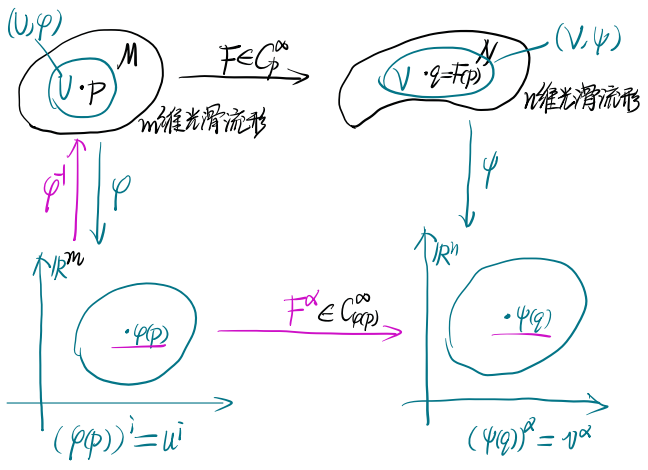
\includegraphics[width=.5\linewidth]{figures/11.png}
            \caption{余切空间图示}
            \label{fig:cotangent space}
        \end{figure}
    \end{enumerate}
\end{remark}
\subsubsection*{切空间}
\begin{itemize}
    \item 切空间 $T_p=\{\langle [\gamma], (\dd f)_p\rangle, \gamma\in \Gamma_p\}$.
    \item 自然基底 $\{[\lambda_k],1\leqslant k\leqslant m\}=\left\{\left(\frac{\partial}{\partial u^k}\right)_p, 1\leqslant k\leqslant m\right\}$.
    \item 切空间之间的光滑映射 ($F^*$的共轭映射)(也称为相伴映射)
    \[F_*\colon T_p\to T_q,\]
    \begin{itemize}[label=\twicecircle]
        \item 作用方式: $\langle F_* X,\alpha\rangle=\langle X,F^* \alpha\rangle, X\in T_p,\alpha\in T_q^*$.
        \item 在两个自然基底下的矩阵表示
        
        切映射$F_*$在自然基底$\left\{\frac{\partial }{\partial u^i}\right\}$上的作用是
        \begin{eq}
            \langle F_*\left(\frac{\partial }{\partial u^i}\right),\dd v^\alpha\rangle &=\lan{\frac{\partial}{\partial u^i},F^*(\dd v^\alpha)}\\ 
            &=\sum_{i=1}^{m}\lan{\frac{\partial }{\partial u^i},\dd u^i}\cdot \left(\frac{\partial F^\alpha}{\partial u^i}\right)_p\\ 
            &=\lan{\sum_{i=1}^{m}\left(\frac{\partial F^\beta}{\partial u^i}\right)_p \frac{\partial }{\partial v^\beta},\dd v^\alpha}.
        \end{eq}
        即 $F_*\left(\frac{\partial }{\partial u^i}\right)=\sum_{\beta=1}^{m}\left(\frac{\partial F^\beta}{\partial u^i}\right)_p \frac{\partial }{\partial v^\beta}$.
    \end{itemize}
        \item 切向量的自然基底表示
        \[[\gamma]=X=\sum_{i=1}^{m}\xi^i \frac{\partial }{\partial u^i}, \xi^i=\frac{\dd (u^i\circ v)}{\dd t},\gamma\in \Gamma_p.\]
        \item 坐标变换
        
        设有另一局部坐标$u^{*i}$,则
        \begin{eq}
            X &=\left(\frac{\partial }{\partial u^1},\cdots,\frac{\partial }{\partial u^m}\right)\overrightarrow{\ell}, \overrightarrow{\ell}=\left(\xi^1,\cdots,\xi^m\right)^\prime\\ 
            &=\left(\frac{\partial }{\partial u^{*1}},\cdots,\frac{\partial }{\partial u^{*m}}\right)\overrightarrow{\ell^*}, \overrightarrow{\ell}=\left(\xi^{*1},\cdots,\xi^{*m}\right)^\prime
        \end{eq}
        由于 $\left(\frac{\partial }{\partial u^{*1}},\cdots,\frac{\partial }{\partial u^{*m}}\right)=\left(\frac{\partial }{\partial u^1},\cdots,\frac{\partial }{\partial u^m}\right)T$,故 $T\overrightarrow{\ell^*}=\overrightarrow{\ell}\implies \overrightarrow{\ell^*}=T^{-1}\overrightarrow{\ell}$,其中$T=\left(\frac{\partial u^{*j}}{\partial u^i}\right)_{(ij)}$,故 $\xi^{*j}=\sum_{i=1}^{m}\left(\frac{\partial u^{*j}}{\partial u^i}\right)\cdot \xi^i$,从而
        \[\sum_{j=1}^{m}\left(\partial \frac{u^{*i}}{\partial u^j}\cdot \xi^j\right)=\sum_{i=1}^{m}\left(\partial \frac{u^{*j}}{\partial u^i}\cdot \xi^i\right).\]
\end{itemize}
\begin{thm}
    设 $M$是 $m$维光滑流形, $N$是 $n$维光滑流形, $m<n$,设 $f\colon M\to N$是光滑映射. 若切映射$f_*$在点$p\in M$是非退化的(即$f_*$在点$p$是单一映射,此时$m\leqslant n$且$f_*$的Jacobi矩阵的秩为$m$,即$f_*$的Jacobi行列式非零),则存在点$p$的局部坐标系$(U;u^i)$及点$q=f(p)$的局部坐标系$(V;v^\alpha)$,使得$f(U)\subset V$,且$f|U$可用局部坐标表示为: $\forall x\in U$,有
    \begin{eq}
        \left\{\begin{array}{ll}
            v^i\circ f(x)=u^i (x), & 1\leqslant i\leqslant m,\\ 
            v^\gamma\circ f(x)=0, & m+1\leqslant \gamma\leqslant n.
        \end{array}\right.
    \end{eq}
\end{thm}
\begin{proof}
    设$f$
在点$p$的局部坐标系$(U;u^i)$与点$q$的局部坐标系$(V;v^\alpha)$下表示为
\[v^\alpha=f^\alpha(u^1,\cdots,u^m), 1\leqslant \alpha\leqslant n.\]
假定 $u^i (p)=0,v^\alpha (q)=0$. 因为$f_*$在点$p$是非退化的,则
\[\frac{\partial (f^1,\cdots,f^m)}{\partial (u^1,\cdots,u^m)}\bigg|_{n^i=0}\neq 0.\]
由于$f_*$在点$p\in M$是非退化的,则$f_*$的Jacobi行列式 $\det\left(\frac{\partial f^\alpha}{\partial u^i}\right)\bigg|_{p}\neq 0$.令上述行列式为$J_{m\times n}, 1\leqslant i\leqslant m,1\leqslant \alpha\leqslant n$,且 $m\leqslant n, \operatorname{rank}(J)=m$, 如下图所示
\begin{align}
    \left[
    \begin{tabular}{cccc|c}
        \multicolumn{4}{c}{}& \\
        \multicolumn{4}{c}{非奇异矩阵}&\\ 
        \multicolumn{4}{c}{$\frac{\partial (f^1,\cdots,f^m)}{\partial (u^1,\cdots,u^m)}$}&\\ 
        \multicolumn{4}{c}{}& \\
    \end{tabular}\right]
\end{align}
令$I_{n-m}=\left\{(\omega^{m+1},\cdots,\omega^{n})\mid |\omega^\gamma|<\delta,m+1\leqslant \gamma\leqslant n\right\} (\delta>0)$.
\begin{eq}
    f\colon U\to V & v^\alpha\colon f\to (f^1,\cdots,f^n)\\ 
    p\mapsto f(p)=q & q\mapsto (v^1,\cdots',v^n)
\end{eq}
将 $f(p)$用 $v^\alpha$作局部坐标表示为 
\[v^\alpha=(f(p))^\alpha=(f(u^1,\cdots,u^m))^\alpha=f^\alpha(u^1,\cdots,u^m),1\leqslant \alpha\leqslant n.\]
假定 $u^i (p)=0,v^\alpha (q)=0$, 因为由 $f$诱导的切映射 $f_*$ 是非退化的,即 $m\leqslant n$且$f_*$的Jacobi矩阵秩为$m$,即
\begin{multline*}
    \frac{\partial (f^1,\cdots,f^m)}{\partial (u^1,\cdots,u^m)}\neq 0,J_{m\times n}=\left(\frac{\partial f^\alpha}{\partial u^i}\right)_p=\frac{\partial (f^1,\cdots,f^m,f^{m+1},\cdots,f^n)}{\partial (u^1,\cdots,u^m)},1\leqslant i\leqslant m,1\leqslant \alpha\leqslant n.
\end{multline*}
\end{proof}
\begin{remark}
    扩充行空间为$n$维即引入$n-m$个维度将$(u^1,\cdots,u^m)$扩展为$(u^1,\cdots,u^m,\omega^{m+1},\cdots,\omega^n)$,并且满足
    定义光滑映射 $\widetilde{f}\colon U\times I_{n-m}\to V$,
    \begin{eq}
        \widetilde{f}^i (u^1,\cdots,u^m,\omega^{m+1},\cdots,\omega^n)&=f^i (u^1,\cdots,u^m) (\text{和原来的$f^i$相同}\quad 1\leqslant i\leqslant m),\\ 
        \widetilde{f}^i (u^1,\cdots,u^m,\omega^{m+1},\cdots,\omega^n)&=\omega^\gamma+f^\gamma(u^1,\cdots,u^m),m+1\leqslant \gamma\leqslant n.
    \end{eq} 
    则显然$\widetilde{f}$在$(u^i,\omega^\gamma)=(0,0)$的Jacobi行列式是非退化的,因为 
    \begin{eq*}
    J_{n\times n}^\prime =\left(\frac{\partial(\widetilde{f}^1,\cdots,\widetilde{f}^n)}{\partial(u^1,\cdots,u^m,u^{m+1},\cdots,u^n)}\right)\neq 0,\quad \ell=\left\{\begin{array}{ll}u,&1\leqslant i\leqslant m,\\ \omega,& m+1\leqslant\gamma\leqslant n.\end{array}\right.
    \end{eq*}
    \begin{align}
        |J^\prime|=\begin{vmatrix}
            \frac{\partial \widetilde{f}^1}{\partial u^1} & \cdots &\frac{\partial \widetilde{f}^m}{\partial u^1} & \frac{\partial \widetilde{f}^{m+1}}{\partial u^1} &\cdots & \frac{\partial \widetilde{f}^n}{\partial u^1}\\ 
            \vdots &&\vdots &\vdots &&\vdots\\
            \frac{\partial \widetilde{f}^1}{\partial u^m} & \cdots &\frac{\partial \widetilde{f}^m}{\partial u^m} & \frac{\partial \widetilde{f}^{m+1}}{\partial u^m}& \cdots & \frac{\partial \widetilde{f}^n}{\partial u^m}\\[10pt]
            \frac{\partial \widetilde{f}^1}{\partial u^{m+1}} & \cdots &\frac{\partial \widetilde{f}^m}{\partial u^{m+1}} & \frac{\partial \widetilde{f}^{m+1}}{\partial u^{m+1}} &\cdots & \frac{\partial \widetilde{f}^n}{\partial u^{m+1}}\\ 
            \vdots &&\vdots &\vdots &&\vdots\\
            \frac{\partial \widetilde{f}^1}{\partial u^n} & \cdots &\frac{\partial \widetilde{f}^m}{\partial u^n} & \frac{\partial \widetilde{f}^{m+1}}{\partial u^n}& \cdots & \frac{\partial \widetilde{f}^n}{\partial u^n}
        \end{vmatrix}=\begin{vmatrix}
            A_m & B_{m\times n-m}\\ 
            C_{n-m\times m} & D_{n-m}
        \end{vmatrix}\neq0
    \end{align}
\end{remark}












